\documentclass[smallextended]{svjour3} 
 \usepackage[T1]{fontenc}
\usepackage[utf8]{inputenc}
%\usepackage{fixltx2e}
\usepackage{ifthen,figlatex}
\usepackage{longtable}
\usepackage{float}
\usepackage{wrapfig}
\usepackage{subfigure}
\usepackage{graphicx}
\usepackage[export]{adjustbox}
\usepackage{xspace}
\usepackage{amsmath,amssymb}
\usepackage[french, frenchb]{babel}
\AtBeginDocument{
\definecolor{pdfurlcolor}{rgb}{0,0,0.6}
\definecolor{pdfcitecolor}{rgb}{0,0.6,0}
\definecolor{pdflinkcolor}{rgb}{0.6,0,0}
\definecolor{light}{gray}{.85}
\definecolor{vlight}{gray}{.95}
}
%\usepackage[paper=letterpaper,margin=1.61in]{geometry}
\usepackage{url} \urlstyle{sf}
\usepackage[normalem]{ulem}
\usepackage{todonotes}
\usepackage[colorlinks=true,citecolor=pdfcitecolor,urlcolor=pdfurlcolor,linkcolor=pdflinkcolor,pdfborder={0 0 0}]{hyperref}
\usepackage[round-precision=3,round-mode=figures,scientific-notation=true]{siunitx}
% \usepackage{minted}
% \usepackage{verbments}
% \usepackage{verbatim}
% \usepackage{alltt}

  \usepackage{graphicx}
  \usepackage{hyperref}
\date{\today}
\title{}
\hypersetup{
  pdfkeywords={},
  pdfsubject={},
  pdfcreator={}}
\begin{document}

\newcommand{\AL}[2][inline]{\todo[color=green!50,#1]{\sf \textbf{AL:} #2}\xspace}
\newcommand{\LS}[2][inline]{\todo[color=green!50,#1]{\sf \textbf{LS:} #2}\xspace}

\let\oldcite=\cite
\renewcommand\cite[2][]{~\ifthenelse{\equal{#1}{}}{\oldcite{#2}}{\oldcite[#1]{#2}}\xspace}
\let\oldref=\ref
\def\ref#1{~\oldref{#1}\xspace}
\def\ie{i.e.,\xspace}
\def\eg{e.g.,\xspace}
\def\qrmspu{\texttt{QRM\_StarPU}\xspace}
\sloppy

\title{Modelisation et simulation d'applications dynamique pour plateformes Exascale%\thanks{Grants or other notes
%about the article that should go on the front page should be
%placed here. General acknowledgments should be placed at the end of the article.}
}
%\subtitle{Do you have a subtitle?\\ If so, write it here}

%\titlerunning{StarPU SMPI}        % if too long for running head

\author{Steven QUINITO MASNADA  \\ \\
        Encadrants : Arnaud LEGRAND \and Luka STANISIC  %if many names separate them with \and.
}

%\authorrunning{Steven QUINITO MASNADA} % if too long for running head

\institute{F. Author \at
              first address \\
              Tel.: +123-45-678910\\
              Fax: +123-45-678910\\
              \email{fauthor@example.com}           %  \\
%             \emph{Present address:} of F. Author  %  if needed
           \and
           S. Author \at
              second address
}

\date{Juin 2015}
% The correct dates will be entered by the editor

\maketitle


\begin{abstract}
Dans le domaine des supercalculateurs, la course à la performance est
un point crucial. Actuellement, le calculateur le plus puissant (le
TianHe-2) est capable d'effectuer environ 33.86 Peta d'opérations
flotantes par secondes. Cependant cette course est freinée par un
facteur qui prend désormais d'une importance capitale, le coût
énergétique. En effet, reprennons l'exemple du supercalculateur
chinois, la consommation du TianHe-2 atteint presque les 18MW et
avec la génération exascale la consommation estimée sera entre 20MW
et 40MW. Dans l'état des fait, ce n'est pas réalisable et pour
pouvoir atteindre l'exaflops, il nécessaire d'optimiser d'autres
points que la puissance des puces. Evidemment des optimisations
peuvent être faites au niveau matériel afin de réaliser des
composants à hautes efficacités énergétiques. On peut également
optimiser le rendement en utilisant au mieux les capacités du
matériel. Cette optimisation ce fait donc du côté logiciel et pour
cela il nous faut  envisager un changement de méthode programmation,
c'est cette dernière que nous allons étudier. L'objectif de mon
stage au sein de l'équipe MESCAL, sous la tutelle d'Arnaud Legrand,
est donc de tenter de mesurer le gain d'une telle solution. 


Dans cette optique, en nous basant sur les standards de
programmation en HPC, nous verrons comment nous pourrions évaluer
les performances d'un nouveau paradigme programmation.
\end{abstract}

\section{Introduction}
\label{sec-1}

La majorité des supercalculateurs actuels, comme le montre le site
\url{http://www.top500.org} sont des clusters massivement parallèles et
souvent de type hétérogènes(CPU-GPU). De ce fait certains standard
ce sont imposés.

Il y a tout d'abord la norme MPI (Message Passing Interface),
qui est une API de communication basée sur l'envoi et la
récéption de message. Elle réputée pour être performante et
portable, et elle est de plus haut niveau que les sockets.

Ensuite, il y a l'API OpenMP qui est une interface de
multihreading de plus haut niveau de PThread. Elle permet de
découper facilement des traitements mais cependant elle ne permet
d'avoir de contrôle sur la priorité des threads, comme cela reste à
la charge de l'ordonnanceur du noyau. 

Enfin, l'API CUDA permet tirer partie de la puissance de calcul
des GPU. Pour cela il est nécessaire de spécifier explicitement de
ce que l'on veut envoyer aux GPUs et on doit également gérer la
synchronisation.  

Si l'on veut optimiser le rendement d'une application afin que
celle-ci tire partie de toute la puissance disponible, il faut faire
en sorte d'occuper au maximum le plus d'unités de calculs possible.  
Le problème est que l'on se retrouve à devoir utiliser plusieurs
paradigme à la fois ce qui complique grandement la programmation.

Généralement, on procède soit en déléguant tous les calculs aux
GPUs, laissant les CPUs en idle. Soit on réparti la charge entre les
CPUs et les GPUs de manière complètement statique. L'inconvénient
est que la mise en pratique très difficile car il est ardu de
trouver un bon équilibrage.

Cependant même si l'on arrive à équilibrer les charges
correctemment, on peut avoir des cas où certaines unités de
calculs ne sont pas occupées alors qu'elles le pourraient. Cela se
produit quand par exemple lorsque certaines unités de calculs
attendent la terminaisons de certain traitements alors que
d'autres auraient put être effectuer en attendant. Cela est dû au
fait que l'exécution soit statique et ce qui induit un idle time
artificiel. De plus cette solution n'est pas portable car le
découpage des traitements ce fait en fonction de la plateforme
cible.

La solution serait donc d'avoir une gestion dynamique des
charges. Mais cela s'avère bien plus ardu, voir impossible
à réaliser directement avec ces méthodes de programmation. Alors
essayons en une autre.

La librairie StarPU est un système runtime qui permet une
répartition des traitements de manière dynamique et opportuniste. 
Pour ce faire elle introduit un nouveau paradigme basé sur les
tâches. StarPU génère un graphe de dépendance permettant
d'optimiser le l'ordonnancement de ces dernières.

La première version de StarPU a été conçu spécialement pour des
architectures hybrides. Une version récente (StarPU MPI) a été
réalisée pour bénéficier d'un ordonnance et d'une exécution qui
soit à la fois dynamique et opportunistes dans un contexte
distribuée afin de répartir la charge entre les différents
noeuds.

Nous allons donc voir comment évaluer les performances
d'applications basés sur StarPU MPI.

Pour cela nous verrons, dans une première partie, les différentes
approches pour l'évaluation de performances d'applications en HPC et
pourquoi nous avons choisi le simulateur Simgrid. Dans une seconde
partie, nous examinerons en détail Simgrid et StarPU ainsi que les
différents problèmes que nous avons rencontrés. Après quoi, dans une
troisième parte, nous verrons les méthodes employées pour répondre à
ces problèmes. Dans une quatrième partie, nous aborderons les
modifications apportées à Simgrid afin de pouvoir effectuer les
mesures. Ensuite dans une cinquième partie, nous verrons le
processus de validation de ces changement. Et pout finir, dans une
sixième partie, nous conclurons sur les résultats que nous avons
réussit à obtenir. 

\section{État de l'art}
\label{sec-2}
En HPC, il y a trois grandes approches possible pour évaluer les
performances d'applications.
\subsection{Test sur systèmes réels}
\label{sec-2-1}
Cette approche consiste à lancer la vrai application sur le système
réel afin d'effectuer les mesures. Cependant cette méthode peut se 
révéler très coûteuse et il n'est pas toujours possible d'avoir
accès à la plateforme. De plus comme les expérimentations ne
peuvent être effectuées sur que sur un petit nombre de plateforme
notamment à cause de coût, on ne peut pas vraiment extrapoler les
résultats. Dernier point important, nous n'avons pas de contrôle
sur les décisions d'ordonnancements, d'une exécution à l'autre on
peut avoir des résultats différents ce qui fait que les
expériences ne sont pas reproductibles. 
\subsection{L'approche par rejeu de trace}
\label{sec-2-2}
Cette méthode consiste à exécuter une première fois l'application
sur un système réel pour ensuite pour ensuite rejouer la trace
post-mortem. Elle est couramment employé dans le contexte 
d'application MPI mais est ici totalement inadaptés car nous avons
à faire à des programmes qui sont non déterministes. En effet, on ne
pourra pas connaître les autres actions qu'il était possible
d'effectuer plutôt qu'une autre, ni leurs impacts.
\subsection{La simulation/émulation}
\label{sec-2-3}
On a d'une part la simulation où l'on crée un faux environnement
proche de la réalité et où les actions ne sont pas réellement
effectués. Dans notre cas on simulerait donc la plateforme de même que l'OS. 
Ainsi, les expérimentations peuvent être effectuées à partir de
n'importe quel système, il n'est plus nécessaire d'avoir accès à la
plateforme, ce qui rend cette approche peu coûteuse. 
Par ailleurs il est facile d'extrapoler les résultats car on peut
simuler un nombre important de plateformes. Ensuite la simulation
permet d'avoir un temps d'exécution plus court qu'avec des tests
réels car on n'effectue que certains traitements ce qui nous permet
pouvoir effectuer un grand nombre de mesures.  
Enfin comme la simulation nous permettrait d'avoir un contrôle sur
l'ordonnancement, nous pourrions avoir un système déterministe qui
nous permettrait d'avoir des expériences qui peuvent être reproduites.

Et on a d'autre part l'émulation où l'on exécuterait en vrai le
programme sur le système simulé. Ainsi, seul le runtime de StarPU sera
réellement exécuté, nous pourrons donc étudier son impact sur le
performances dans un contexte MPI.

C'est pour ses divers avantages que nous avons opter pour la
simulation / émulation. Le logiciel qui a été choisi est Simgrid, 
un simulateur de systèmes distribués, de grilles de calculs, de
systèmes peer to peer et cloud.
De plus StarPU a récemment été portée au-dessus de Simgrid et
concilie l'approche simulation /  évaluation.

\section{Analyse du problème}
\label{sec-3}
\subsection{Simgrid: Les processus}
\label{sec-3-1}
Sous Simgrid, les processus sont modélisés par des threads, ce
qui signifie que leur espace d'adressage est partagé.
Afin que ces derniers ce comportent comme des processus UNIX, il
est nécessaire que chaque processus n'ait pas accès aux
variables d'un autre, c'est pourquoi un système de
privatisation a été mis en place. L'approche est la suivante:
pour chaque processus, une zone mémoire est allouée dans le
tas grâce à un mmap. Cette zone est le nouveau segment données du
processus, et à chaque changement de contexte, on fait pointer
vers cette zone. 

\begin{figure}[htb]
\centering
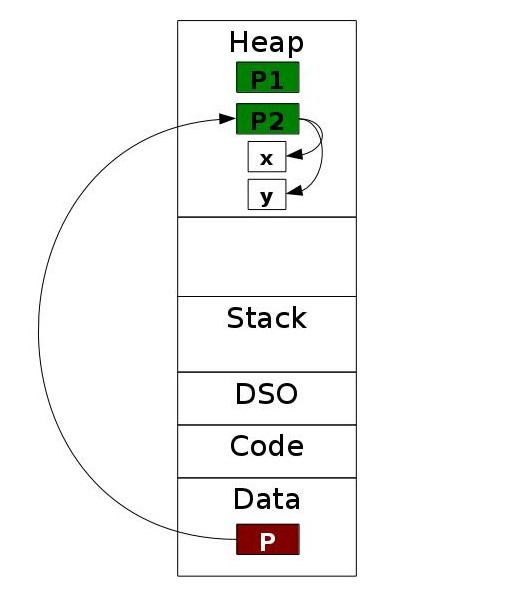
\includegraphics[width=5cm]{./Img/Memoire.jpg}
\caption{\label{fig:1}Privatisation du segment données}
\end{figure}

\subsection{SimGrid/MPI: Architecture générale}
\label{sec-3-2}
Cette API permet de simuler la couche MPI. Actuellement, la majeur
partie des fonctionnalités MPI ont été implémentées. 
Le fonctionnement est le suivant :
\begin{itemize}
\item l'application que l'on veut tester est compilée en remplaçant
le mpi.h classique par le mpi.h de Simgrid
\item à l'édition de lien on remplace le main de l'application par
celui de Simgrid.
\item Ce dernier a pour rôle de préparer l'exécution du simulateur
en créant la plateforme et en déployant les processus SMPI qui
exécuterons chacun le main de l'application MPI.
\end{itemize}

\subsection{StarPU-SG: Architecture générale}
\label{sec-3-3}
StarPU a été modifié afin de pouvoir fonctionner au dessus du
simulateur Simgrid et est basé sur l'API MSG. L'application est
exécutée réellement mais les allocations mémoires des tâches ne
sont pas effectuées, les codes de calcul sont simulés et remplacés
par un délais de même pour les transferts CUDA.

\subsection{Ce qui coince}
\label{sec-3-4}
Comme en MPI on est dans un contexte d'espace mémoire distribuée,
les processus MPI d'un même noeud doivent partager les données donc
il faut faire en sorte que le segment data d'un processus soit
rattaché à celui qui les a crées. Or, comment concilier à la fois
la privatisation du segment données entre les processus de noeud
différents et le partage entre les processus d'un même noeud?

De plus, une autre difficulté vient du fait qu'à la base MSG et
SMPI n'ont pas été prévus pour fonctionner en ensemble. il nous
faut arriver à correctement initialiser en la partie MSG et SMPI.

\section{Méthodologie}
\label{sec-4}
Comme nous travaillons avec Simgrid et StarPU à la fois, nous
utilisons un dépôt complexe comprenant les deux et gérer avec
l'outils submodule de git. Ce dernier nous permet de gérer des sous
dépôt indépendemment, ainsi il est plus aisé de traiter les mises à
jours de ces derniers.

Afin de pouvoir retracer le cheminement de mon travail, mais aussi
de pouvoir garder le fil d'un jour à l'autre, un cahier de
laboratoire est tenu en org-mode et est hébergé sur github. Cela permet
également à mon tuteur de stage de savoir chaque jours l'avancement
du projet et des difficultés rencontrées.

Comme on l'a vu précédemment il est nécessaire d'apporter quelques
modifications au niveau du simulateur. Dans ce but, il a été dans un
premier temps nécessaire de consulter la documentation afin de
comprendre le fonctionnement et l'architecture de Simgrid. Ensuite
il a fallut explorer le code afin de déterminer où et comment
apporter les modifications. Pour cela les outils tels que GDB,
Valgrind, les etags et CGVG ont été d'une aide précieuse.

\section{Contribution}
\label{sec-5}
La toute première chose à réaliser afin de pouvoir effectuer des
mesures, a été la gestion du partage du segment de données au niveau
du simulateur dans un contexte SMPI. Comme la mémoire est partagée
au sein d'un noeud, nous avons fait en sorte que les processus d'un
même noeud aient leurs segment données en commun. Le principe est le
suivant, il y a dans un premier temps, les processus SMPI qui sont
créés au lancement de l'application avec leur propre espace de
données. Puis ces dernier peuvent à leurs tours créer de nouveau
processus. Ceux-ci héritent donc du segment de données du processus
qui les a créés. Nous avons donc fait pointés le segment données des
processus fils sur celui du père et un échange est effectué au
changement de contexte.

Une fois la gestion du partage mise en place, nous avons constaté
qu'il y avait un cas que nous n'avions pas pris en compte: celui des
librairies dynamiques. Voici comment sont stockés les bibliothèques
en mémoire:

\begin{figure}[htb]
\centering
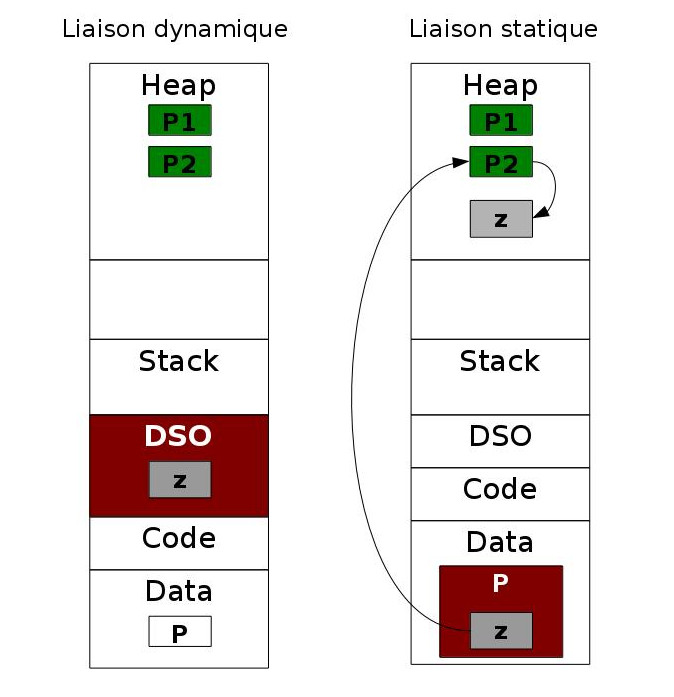
\includegraphics[width=5cm]{./Img/StaticDyn.jpg}
\caption{\label{fig:2}Emplacement en mémoire des bibliothèques}
\end{figure}

En effet, nous n'avons privatisé que le segment données des
processus or, les variables globales des librairies dynamiques (DSO
sur le schéma ci-dessous) ne se trouvent pas dans le segment données
du processus et se retrouvent donc accessible à tous les processus. 

La solution qui nous avons employé est d'utiliser donc une version
statique de la librairie. Ainsi, les variables globales se
retrouvent dans le segment données du processus et ainsi la
privatisation et le partage s'effectue grâce au mécanisme
précédent. Cependant cette solution comporte une limitation car elle
nécessite de changer la chaîne de compilation des applications
utilisant StarPU, mais cela sera suffisante pour effectuer nos tests. 

\section{Validation}
\label{sec-6}
\subsection{Test simple}
\label{sec-6-1}
Dans le but de tester le bon fonctionnement des modifications
apportées, un test illustrant le fonctionnement de StarPU a été
fourni et enrichi. Ce dernier permet ainsi d'isoler le problème
afin de pouvoir nous concentrer dessus. Ce test, initialise Simgrid
et la partie SMPI comme cela est fait du côté de StarPU et fait
appel à une bibliothèque dynamique et manipule des variables
globales. Ainsi lors de l'exécution de ce test, on doit pouvoir
constater que pour des processus appartenant à un même noeuds, les
valeurs des variables globales du programme et des bibliothèques
dynamiques sont bien identiques. Ce qui après plusieurs correction
a été le cas.  
\subsection{Test de StarPU - SMPI}
\label{sec-6-2}
Comme les résultats du test simples étaient ceux attendu, nous
sommes passé à un test utilisant cette fois la vrai bibliothèque
StarPU. Cette dernière est fourni avec des exemples de programme MPI
notamment d'algèbre linéaire tel que l'algorithme de Cholesky. Nous
nous sommes servi de ces dernier afin de valider les
modifications. Cependant, malgré les ajouts apportés au test, ce 
dernier était incomplet et il semble qu'il y a avoir des soucis au
niveau de  l'initialisation de Simgrid côté StarPU.

\section{Conclusion}
\label{sec-7}
Pour conclure, nous avons voulu voir s'il était possible de mesurer
l'influence d'un runtime dynamique sur les performances
d'applications MPI. Parmi les différentes techniques de mesures de
performances, nous avons fait le choix de la simulation / émulation
car elle nous semble la plus avantageuse, en raison de son coût,
mais aussi en terme de scalabilité.  

Pour vérifier si cette approche est effectivement possible, nous
avons modifié Simgrid afin de pouvoir faire fonctionner StarPU MPI
dessus. Nous avons donc mis en place le partage du segment données
entre les processus de même noeud et la privatisation entre les
processus de noeuds différents. 

Malheureusement par manque de temps il n'a pas encore été possible
de corriger le problème d'initialisation et donc les mesures prévues
n'ont pas encore pu être réalisées. Bien qu'aucune expérimentation
n'est pu être faite, les problèmes rencontrés sont plutôt des
problèmes d'ordre techniques et ne nous permettent pas d'invalider
notre hypothèse. 

Afin de pouvoir conclure sur la question, il faudra finir de
corriger la phase d'initialisation côté StarPU et également apporter
quelques correctifs à Simgrid\cite{MPI}. Ensuite nous pourrons effectuer les
simulations et les mesures. Pour ce faire les mesures seront faites
sur le logiciel Chameleon (un solveur d'algèbre linéaire basé sur
StarPU). Enfin, dans le but de valider le résultat des
expérimentations, un test grandeur nature sera fait sur Grid5000.


\section*{Acknowledgments}
Je souhaite remercier\ldots{}

%\nocite{*}
\def\raggedright{}
\bibliographystyle{IEEEtran}
\bibliography{biblio}
\end{document}